\section{数据理解与总体框架}

\subsection{数据和参数来源}

表~\ref{tab:data-source} 给出四问所需信息及其用途。题面给出的干基含水率定义为单位干物质质量对应的水质量，后续守恒关系和平均含水率计算必须沿用这一口径。

\begin{table}[H]
  \centering
  \caption{数据、经验公式与模型用途}
  \label{tab:data-source}
  \begin{tabularx}{\textwidth}{p{0.16\textwidth}p{0.30\textwidth}X}
    \toprule
    来源 & 主要内容 & 用途 \\
    \midrule
    题面 & 几何尺寸、初始温度 $28\,{}^\circ\mathrm{C}$、初始含水率 $2.55\,\mathrm{kg/kg}$ & 初始区域和初始条件 \\
    附件~1 & 烘房温度与水分浓度的时间序列 & 表面热、湿边界及阶段划分 \\
    附件~2 & 药材半径随时间的变化 & 问题四的移动边界 $R(t)$ \\
    附件~3 & 四个结果文件模板 & 输出时间、空间网格和工作表格式 \\
    附录~2 & 问题一的常物性和对流参数 & 预热阶段固定参数模型 \\
    附录~3 & 问题二、三的变物性经验公式 & 全过程热湿演化和达标判断 \\
    附录~4 & 问题四的变物性经验公式 & 收缩区域上的热湿演化 \\
    \bottomrule
  \end{tabularx}
\end{table}

\subsection{预处理和统一口径}

附件数据进入模型前统一转换为 SI 单位：半径由厘米换算为米，摄氏温度在经验式中换算为开尔文，时间统一以秒存储、在论文表格中按题目要求换算为小时。离散时间之外的烘房边界和半径通过\resultblank{待选择的插值方法}计算，并检查插值是否引入超出原始范围的振荡。

所有结果先按完整精度计算，再在 Excel 和论文表格的最终输出环节统一保留四位小数。代码输出、结果报告和论文表格使用同一份数据源，避免多次人工复制带来口径差异。

\draftnote{收到附件后补充数据规模、采样间隔、缺失和异常情况。未经 EDA 核对前，不在正文声称数据连续、无异常或满足某种函数形式。}

\subsection{四问的模型递进}

四问的求解顺序如图~\ref{fig:framework} 所示。

% Source: figures/流程图.svg; converted to vector PDF for XeLaTeX.
\begin{figure}[H]
  \centering
  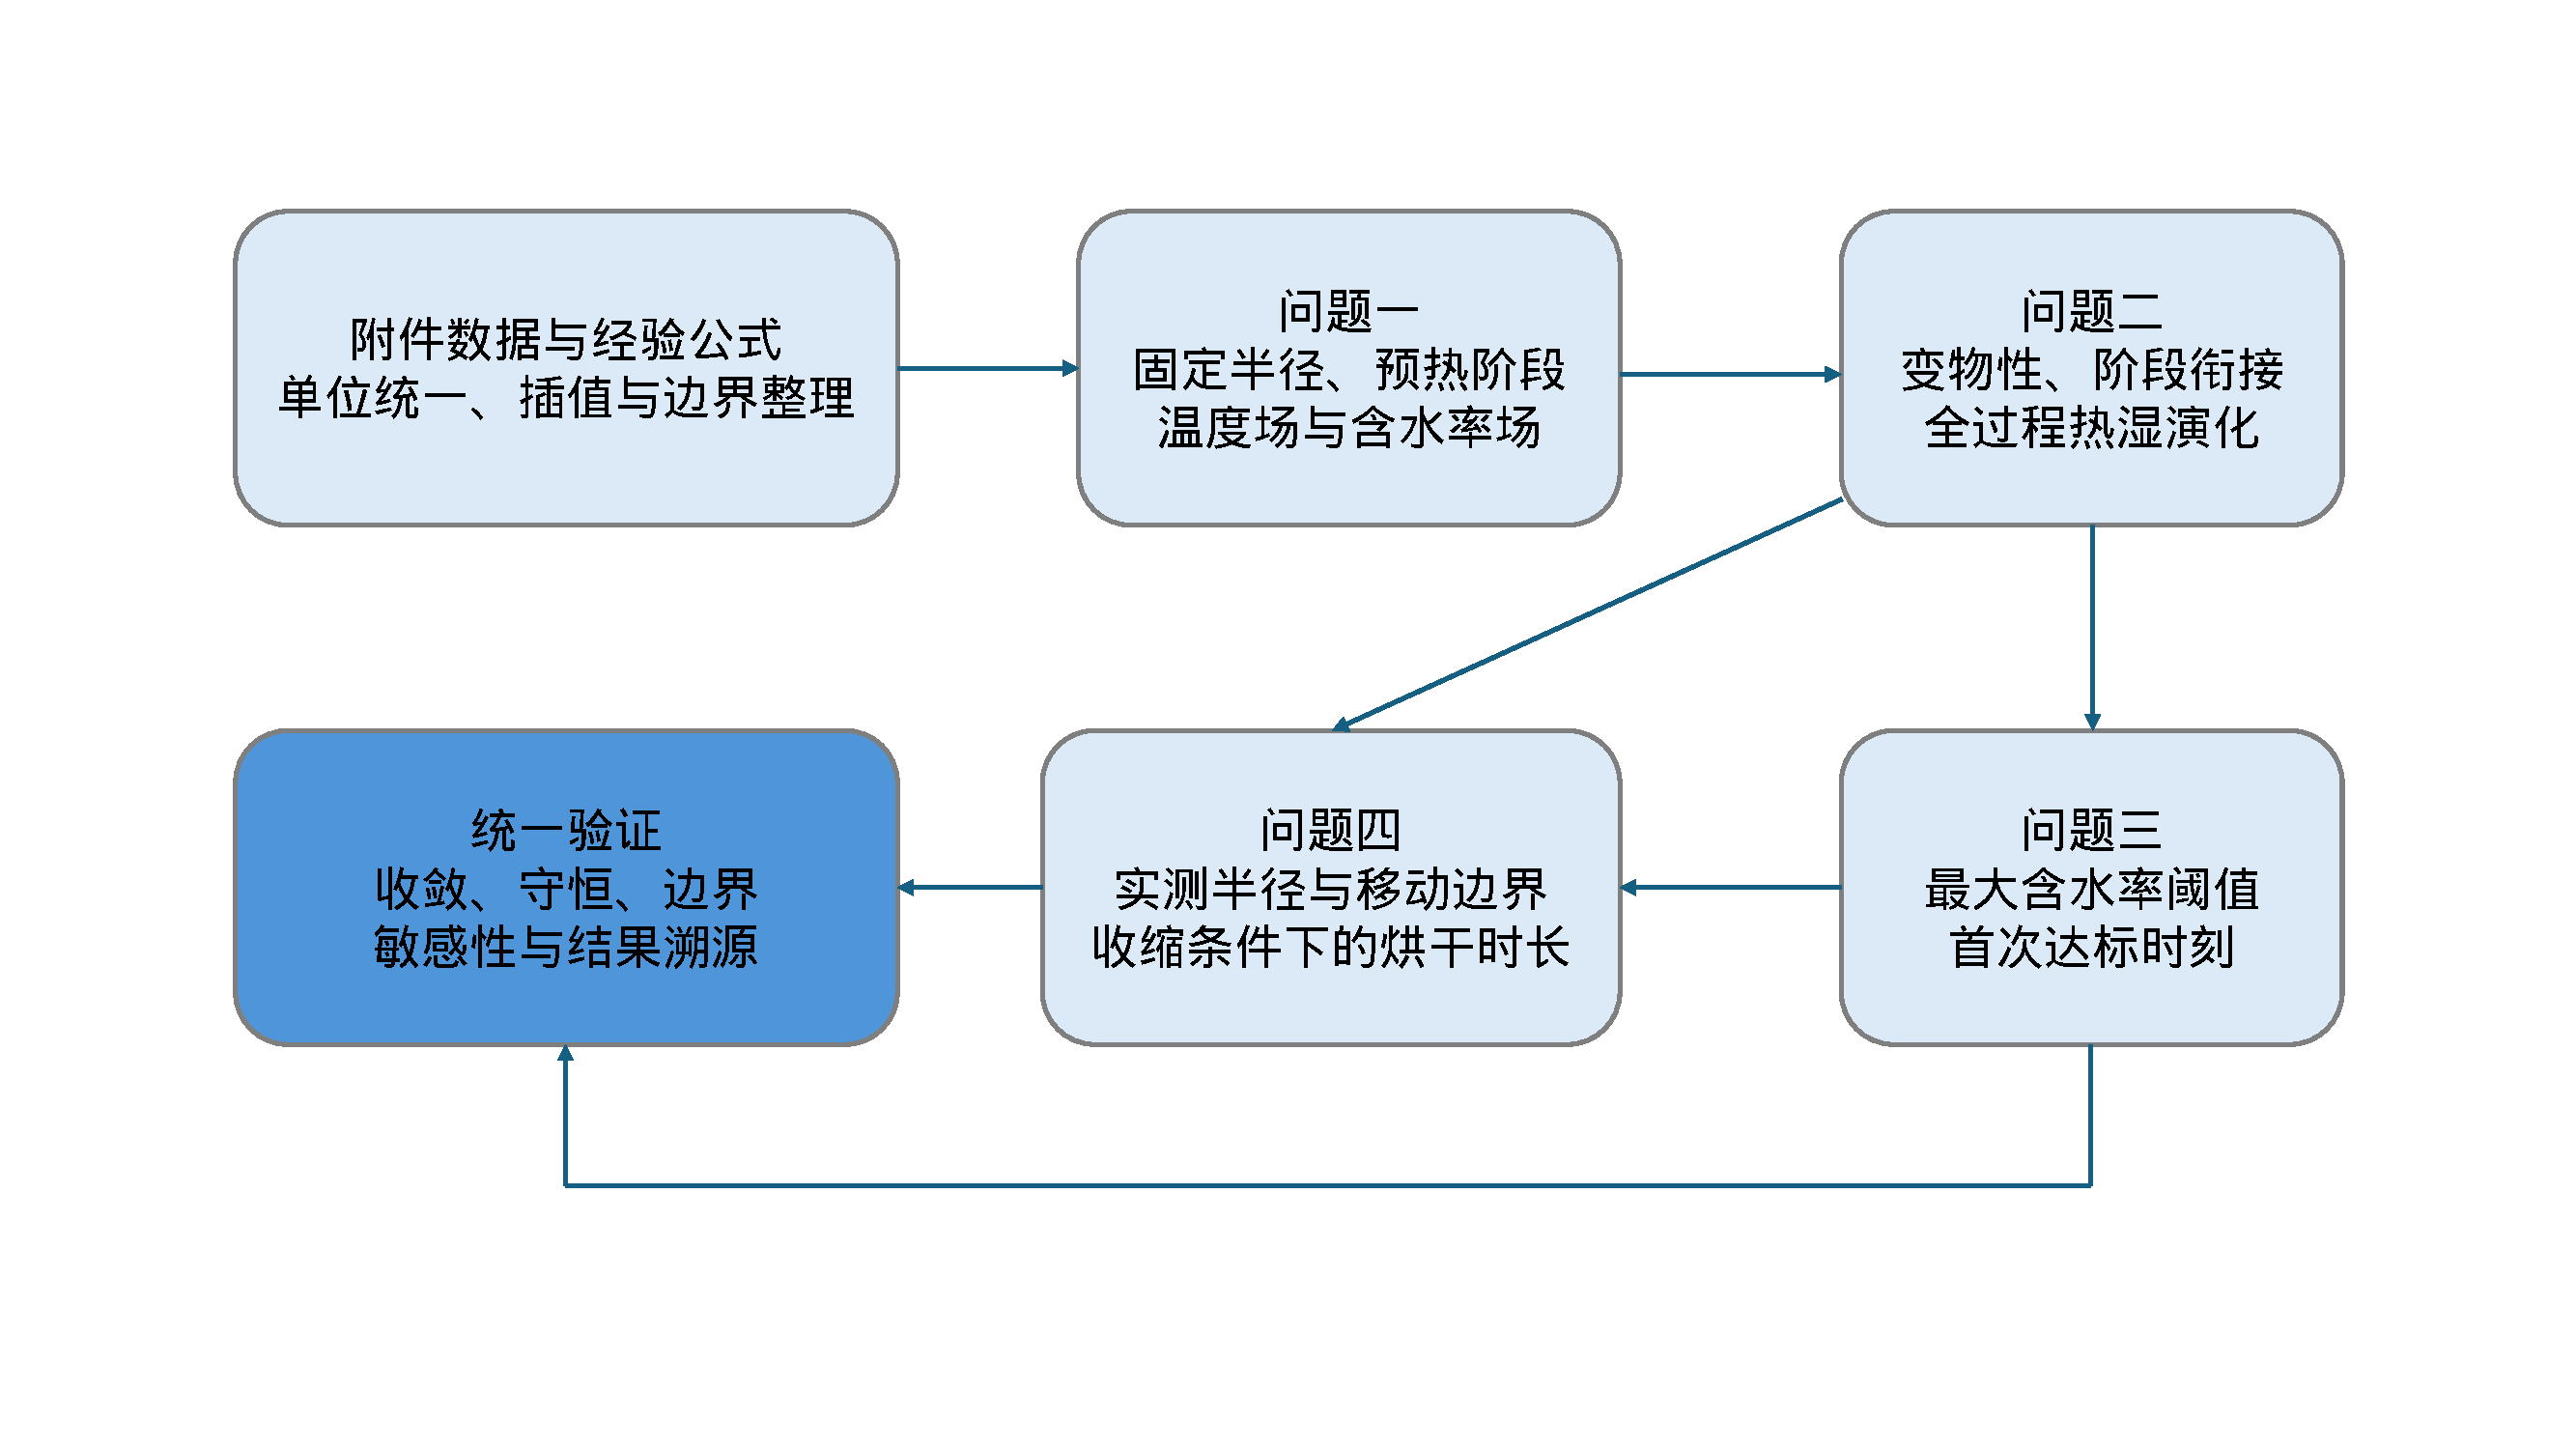
\includegraphics[width=\textwidth]{figures/model_flowchart.pdf}
  \caption{四问建模流程}
  \label{fig:framework}
\end{figure}


问题二是全题的主干：其状态量和数值求解器被问题三直接复用；问题四则复用其热湿传递结构，但必须重写随半径变化的空间处理。问题三与问题四的烘干时长均通过“整个当前药材区域的最大含水率首次低于阈值”判断。

\subsection{论文结果来源约定}

问题一至问题四的关键表格分别由 \texttt{result1.xlsx} 至 \texttt{result4.xlsx} 的同源数据生成。图表用于解释径向梯度、阶段转换、终点附近变化和收缩影响；论文不直接使用临时计算、聊天记录或手工估算的数值。

